% Open this file as the main document in Overleaf and replace TEAM MEMBER NAMES.
% Upload the five PNGs from results/ to results/ in Overleaf, or put them in figures/.
\documentclass[11pt,letterpaper]{article}
\usepackage[T1]{fontenc}
\usepackage{lmodern}
\usepackage[margin=0.9in]{geometry}
\usepackage{microtype}
\usepackage{amsmath,amssymb}
\usepackage{booktabs,graphicx}
\usepackage[font=small]{caption}
\usepackage{placeins}
\usepackage[hidelinks]{hyperref}

\graphicspath{{figures/}{results/}{../results/}}
\setlength{\intextsep}{8pt plus 2pt minus 2pt}
\setlength{\textfloatsep}{12pt plus 3pt minus 3pt}

\title{VAE vs.\ DCGAN: Comparing Fidelity and Diversity on Fashion-MNIST}
\author{TEAM MEMBER NAMES}
\date{COMP 4102 Final Project}

\begin{document}
\maketitle

\section{Problem and motivation}

We wanted to see what two image generators learn when they are trained on the
same clothing images. The main questions were which model makes sharper
images, which covers more of the types of images in the dataset, and which
changes more evenly when we move between two points in its latent space.
These are separate questions. A sample can look convincing even if the
generator mostly makes the same few types of clothes.

We compared a variational autoencoder (VAE) and a deep convolutional
generative adversarial network (DCGAN). We used the same convolutional
design for both image-producing networks so we could focus on the effect of
their training methods. We expected the DCGAN to make sharper images because
it learns from a discriminator that can use edges and texture. We also
expected the VAE to change more gradually along a latent path because it
learns to put its codes near a shared prior. For coverage, we wanted to see
whether the DCGAN would favour a few classes or learn a fairly balanced mix.

\section{Method}

\subsection{Variational autoencoder}

The VAE learns to encode an image and then reconstruct it
\cite{kingma2014}. Given an image \(x\), the encoder produces two vectors,
a mean \(\mu(x)\) and a log-variance \(\ell(x)=\log\sigma^2(x)\). Here each
vector has 32 entries. Together they describe a Gaussian distribution for
the latent code. We get the standard deviation by taking
\(\exp(\ell/2)\), which stays positive. We then sample the code and decode
it to get a reconstruction \(\hat{x}\).
\[
  \varepsilon \sim \mathcal{N}(0,I),
  \qquad
  z = \mu(x) + \exp\bigl(\ell(x)/2\bigr)\odot\varepsilon.
\]
Here \(\odot\) means element-wise multiplication. Drawing \(\varepsilon\)
separately lets gradients reach the mean and log-variance through the
scale and shift. This is the reparameterization trick.

The loss per image combines the squared reconstruction error and the KL
divergence from the standard normal prior. The training code averages the
loss over the batch.
\[
  \mathcal{L}_{\mathrm{VAE}} =
  \underbrace{\lVert x-\hat{x}\rVert_2^2}_{\text{reconstruction}}
  + \underbrace{\frac{\beta}{2}\sum_{j=1}^{32}
    \left(\mu_j^2 + \exp(\ell_j)-1-\ell_j\right)}_{\text{KL penalty}},
  \qquad \beta=1.
\]
The pixel sum keeps the reconstruction loss on the intended scale
relative to the KL penalty. The KL term encourages codes that the decoder
can work with when we draw new noise from \(\mathcal{N}(0,I)\).
If several plausible images have similar codes, an
average image can have low squared error. This gives the decoder a reason
to smooth out details such as folds or straps.

\subsection{Deep convolutional GAN}

The DCGAN has a generator \(G\) that takes random noise \(z\) and a
discriminator \(D\) that estimates whether an image is real
\cite{goodfellow2014,radford2016}. The original GAN describes training as a
minimax game.
\[
  \min_G \max_D\ \Bigl(
  \mathbb{E}_{x\sim p_{\mathrm{data}}}\!\left[\log D(x)\right]
  + \mathbb{E}_{z\sim\mathcal{N}(0,I)}
      \!\left[\log\bigl(1-D(G(z))\bigr)\right]
  \Bigr).
\]
Here \(D(x)\) is the probability after a sigmoid. Our code works with the
scores before the sigmoid and uses binary cross-entropy with logits. We
update the discriminator with real and generated images first. The
generated images are detached for that update, so only the discriminator
weights change. We then update the generator with the non-saturating loss
proposed in the GAN paper.
\[
  \mathcal{L}_{G} =
  -\mathbb{E}_{z\sim\mathcal{N}(0,I)}\!\left[\log D(G(z))\right].
\]
This loss gives a stronger learning signal when the discriminator can
easily spot fake images early in training. The generator gets feedback on
whether an image looks real, so it can learn to keep details that a
pixel-level reconstruction loss might smooth out. The discriminator
judges the samples it sees, which leaves open the possibility that the
generator makes a limited range of convincing images.

\section{Implementation and data}

Fashion-MNIST has 60,000 training images and 10,000 test images across ten
clothing classes \cite{xiao2017}. Each image is grayscale and starts at
\(28\times28\) pixels. We pad the edges with two black pixels to make
\(32\times32\) images. Padding keeps the original edges intact for the
sharpness comparison. We scale the pixel values to \([-1,1]\) to match the
\texttt{tanh} output of the models.

We wrote the model layers and training loops in PyTorch and used
Torchvision to load Fashion-MNIST \cite{pytorch,torchvision}. The VAE
decoder and DCGAN generator have the same layer design and learn their
own weights. They expand a \(4\times4\) feature map to \(8\times8\),
\(16\times16\), and finally \(32\times32\). On the image-reading side we
reuse the design that shrinks the image. The VAE encoder has 64 outputs
for its 32 means and 32 log-variances. The discriminator has one output
for its real-versus-fake score.

Both bundled generators were trained on the training split for 30 epochs
with a batch size of 128, a latent size of 32, and training seed 0. They
use the same weight initialization rule. Both use Adam \cite{adam}. The
VAE uses a learning rate of \(10^{-3}\), and the DCGAN uses
\(2\cdot10^{-4}\) with Adam's first momentum coefficient set to \(0.5\).
The generators train on the images without class labels. A separate
clothing classifier uses the labels for its own training and reached
\(90.7\%\) accuracy on test images.

The training scripts are in \texttt{src/} and read their settings from
\texttt{configs/}. For the experiment in this report, we loaded the
checkpoints from \texttt{trained\_models/}. From the project folder,
\texttt{python compare.py} runs the comparison on CPU and writes the score
table and four comparison figures to \texttt{results/}.

\section{Experiments and results}

\subsection{How we evaluated the models}

We generated 10,000 images per model using the same 32-dimensional noise
vectors. The real reference was the full Fashion-MNIST test split. We also
compared a random set of 10,000 real training images with that test split.
This row gives a reference for the score we get when both sets contain
real clothes.

The classifier gives each image a vector of 128 features. We compute
Fr\'echet distance on these features using the same distance formula as
FID \cite{heusel2017}. A smaller distance means the two sets have more
similar feature statistics. Feature precision asks how many generated
images fall near the real images in feature space. Feature recall asks
how many real images fall near generated samples. We use neighbourhoods
based on the third nearest neighbour \cite{kynkaanniemi2019}.

We also use the classifier to estimate the class mix of the generated
images. Class KL measures how far that mix is from the true class shares
in the test set. For sharpness, we apply a Laplacian edge filter and
average its variance across images \cite{pechpacheco2000}. We use the
real-image row as a guide because noise can also give a high edge score.

For each model we sampled 100 pairs of latent codes and generated 10
frames per pair using spherical interpolation \cite{white2016}. We
measured the distances between neighbouring frames in classifier feature
space. The coefficient of variation (CV) is the standard deviation of
those distances divided by their mean. A lower CV means the steps are
more even. This score describes the size of the changes across a path.

\subsection{Results from the saved checkpoints}

\begin{table}[!htbp]
\centering
\small
\setlength{\tabcolsep}{5pt}
\begin{tabular}{lrrrrrr}
\toprule
Group & FID-clf \(\downarrow\) & Prec. \(\uparrow\) & Recall \(\uparrow\) &
Edge var. & Class KL \(\downarrow\) & Path CV \(\downarrow\) \\
\midrule
Real train & 0.03 & 0.903 & 0.893 & 0.150 & 0.005 & \textemdash \\
VAE        & 21.12 & 0.699 & 0.488 & 0.039 & 0.218 & 0.503 \\
DCGAN      & 1.32 & 0.856 & 0.856 & 0.148 & 0.026 & 0.696 \\
\bottomrule
\end{tabular}
\caption{Comparison on 10,000 images per group. FID-clf uses clothing
classifier features. Edge variance is interpreted relative to the real
row. The exact values are in \texttt{results/metrics.csv}.}
\label{tab:main}
\end{table}

The DCGAN was much closer to the real data in classifier feature space.
The recall was \(0.856\) for the DCGAN and \(0.488\) for the VAE. The
DCGAN's edge score of \(0.148\) was close to the real value of \(0.150\).
The first samples in Figure~\ref{fig:samples} show what those numbers
look like. Several DCGAN samples keep clear hems and outlines, while
the VAE clothes often have softer boundaries.

The real-training row helps put the recall scores in context. Its recall
was \(0.893\), so the DCGAN was about \(3.7\) percentage points below
that reference, and the VAE was about \(40\) points below it. The
real-training row also has a small Fr\'echet distance of \(0.03\).
The training and test photos are different, so the feature statistics
can differ a little even when both groups contain real clothes.

\begin{figure}[!htbp]
\centering
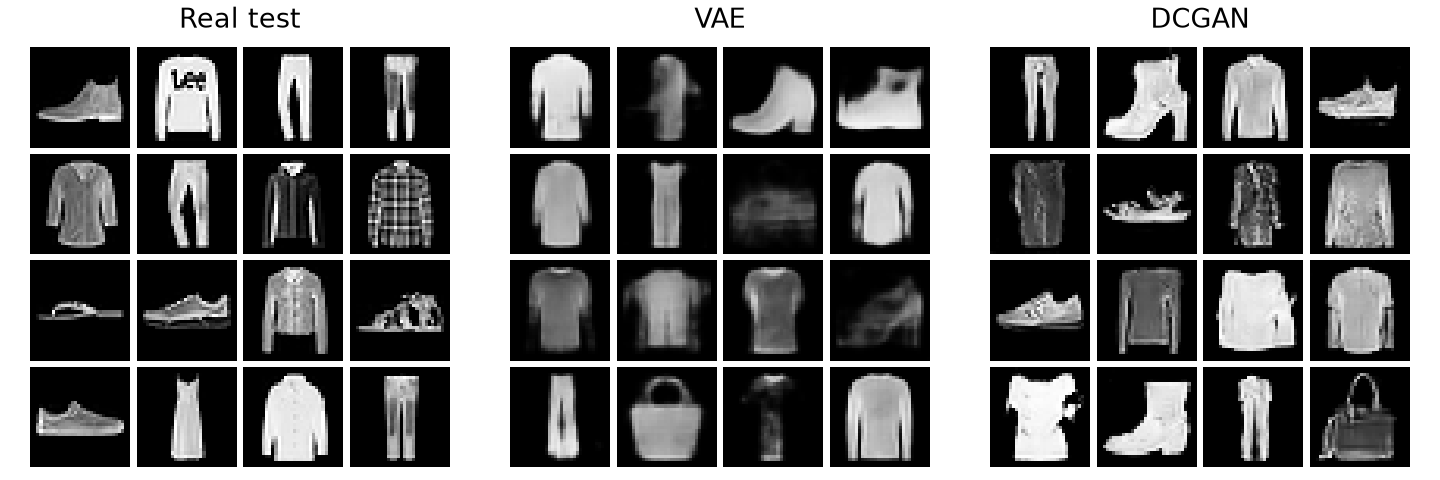
\includegraphics[width=0.97\linewidth]{samples.png}
\caption{The first 16 test images and the first 16 generated samples
from each model. Both generators use the same noise vectors.}
\label{fig:samples}
\end{figure}
\clearpage

\subsection{Training dynamics}

We used the saved logs from the same seed-0 runs to see how each model
changed over the 30 epochs. The top row of Figure~\ref{fig:training}
shows the losses recorded after each epoch. The bottom row uses the
archived checkpoint evaluations from every five epochs. Each checkpoint
evaluation compares 5,000 generated images with 5,000 test images.
Table~\ref{tab:main} uses 10,000 images per group for the final comparison.
Run \texttt{python plot\_training.py} to rebuild the figure from the CSVs
in \texttt{results/training/}.

\begin{figure}[!htbp]
\centering
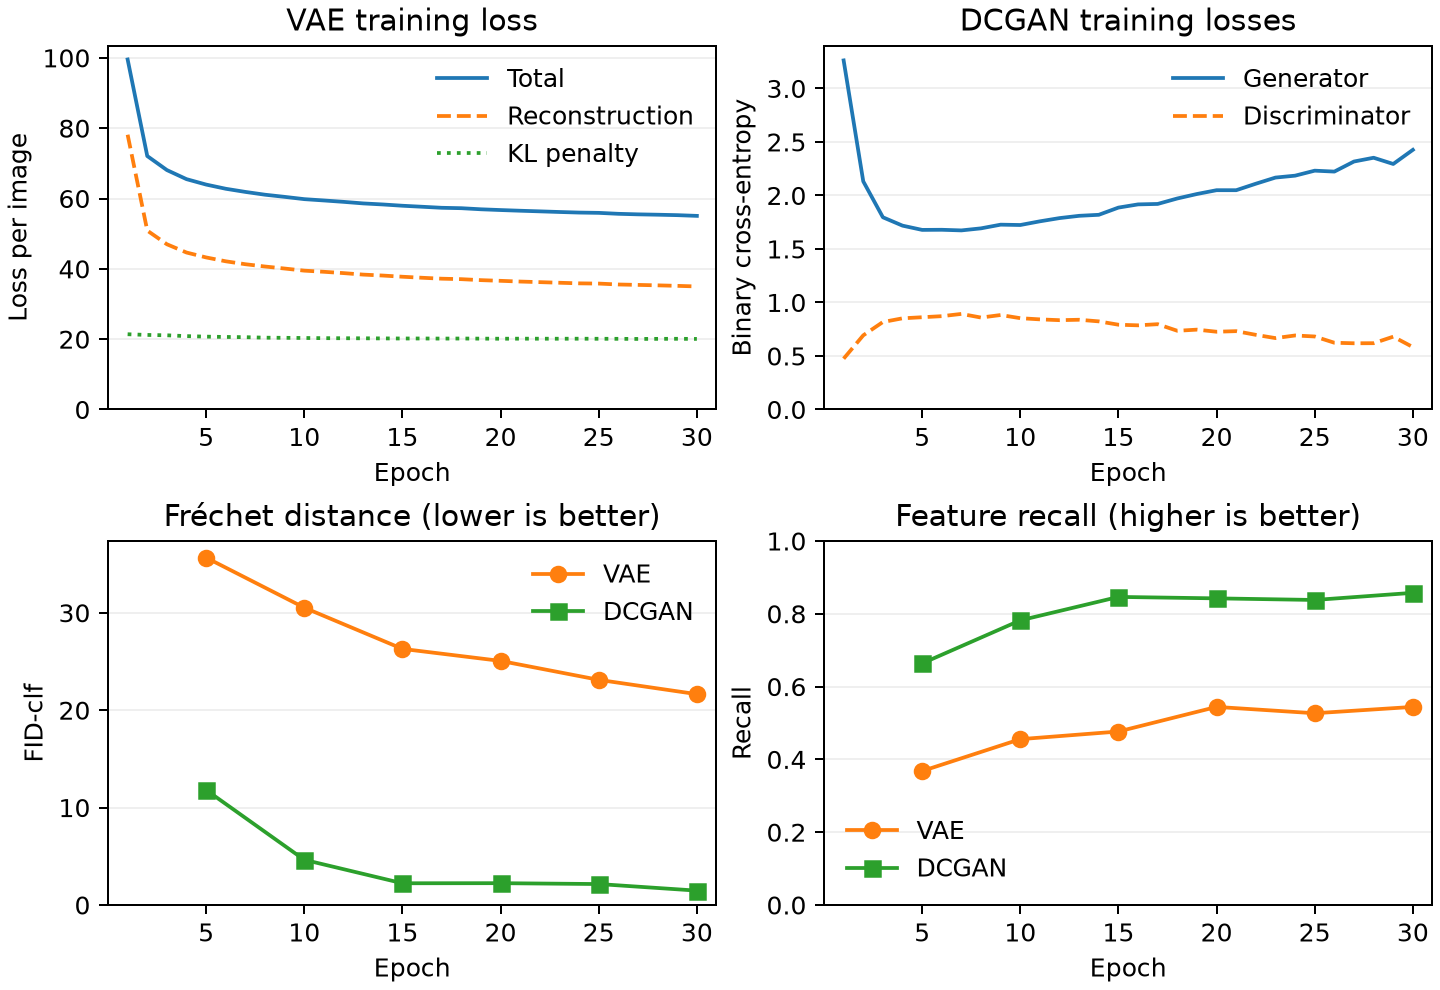
\includegraphics[width=0.97\linewidth]{training_curves.png}
\caption{Training dynamics of the bundled seed-0 runs. The top panels
show each model's training losses on its own scale. The bottom panels
compare both models using the same classifier features.}
\label{fig:training}
\end{figure}
\FloatBarrier

Most of the drop in the VAE loss came from reconstruction error, which
fell from \(78.1\) to \(35.0\) per image. Its KL term stayed near \(20\).
The DCGAN generator loss fell early and rose again later, even as its
generated images got closer to real images in feature space. Both parts
of the GAN are learning during training, so the generator faces a
changing discriminator. The checkpoint scores give us a common way to
compare what the two generators produce.

The DCGAN's Fr\'echet distance fell from \(11.80\) at epoch 5 to \(2.23\)
at epoch 15, then reached \(1.48\) at epoch 30. The VAE improved more
gradually, from \(35.66\) to \(21.65\). Recall rose overall for both runs,
with some dips between checkpoints. The DCGAN finished at \(0.858\)
and the VAE at \(0.544\) in these checkpoint evaluations. This shows
that the gap was already visible early in these two runs.

\clearpage

\section{Analysis and discussion}

\subsection{Coverage and failure cases}

The VAE favoured pullovers and ankle boots and produced relatively few
images classified as coats. The DCGAN's predicted mix was closer to the
balanced real classes (Figure~\ref{fig:balance}). This helps explain
why it had better recall in feature space. The classifier can also
mistake one type of blurry clothing for another, so the bars are best
read together with the sample images.

\begin{figure}[!htbp]
\centering
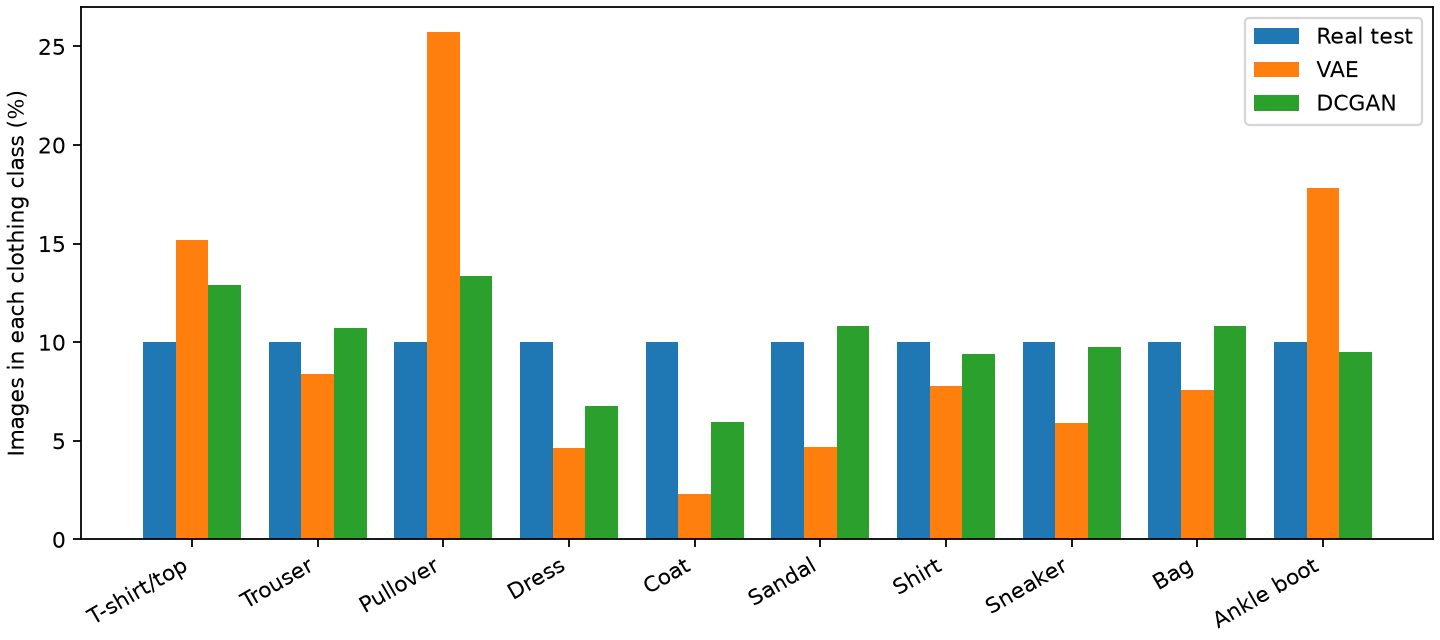
\includegraphics[width=0.83\linewidth]{class_balance.png}
\caption{True class shares for real test images and predicted class
shares for the generated images.}
\label{fig:balance}
\end{figure}

To look at successes and failures consistently, we saved the eight
highest- and lowest-confidence samples for each model
(Figure~\ref{fig:examples}). The VAE often succeeds on trousers, where the
silhouette is clear even with soft edges. Its lower-confidence examples
include faint shapes that are hard to identify. The DCGAN produces
clearer bags and shoes. Some of its low-confidence images have sharp
features but irregular shapes or extra texture. This is why we use the
edge score together with the image grids. Strong edges can also come
from artifacts.

\begin{figure}[!htbp]
\centering
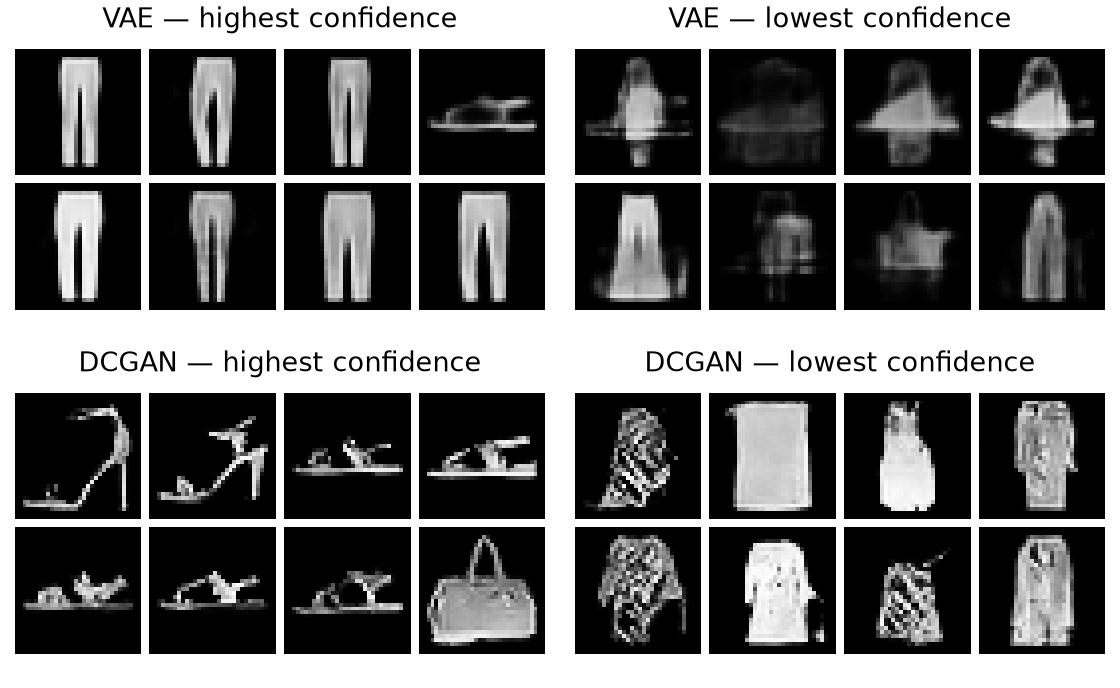
\includegraphics[width=0.74\linewidth]{successes_and_failures.png}
\caption{Examples selected by classifier confidence. The left column
shows high-confidence samples, and the right column shows low-confidence
samples.}
\label{fig:examples}
\end{figure}
\FloatBarrier

\subsection{Latent paths and limits}

The VAE had the more even interpolation steps, with a CV of \(0.503\)
against \(0.696\) for the DCGAN. Figure~\ref{fig:paths} shows one example.
The VAE changes a light top gradually, while the DCGAN makes a larger
change near the end of its path. Both models can move between images
along a path. The score compares how evenly that change is spread across
the frames.

\begin{figure}[!htbp]
\centering
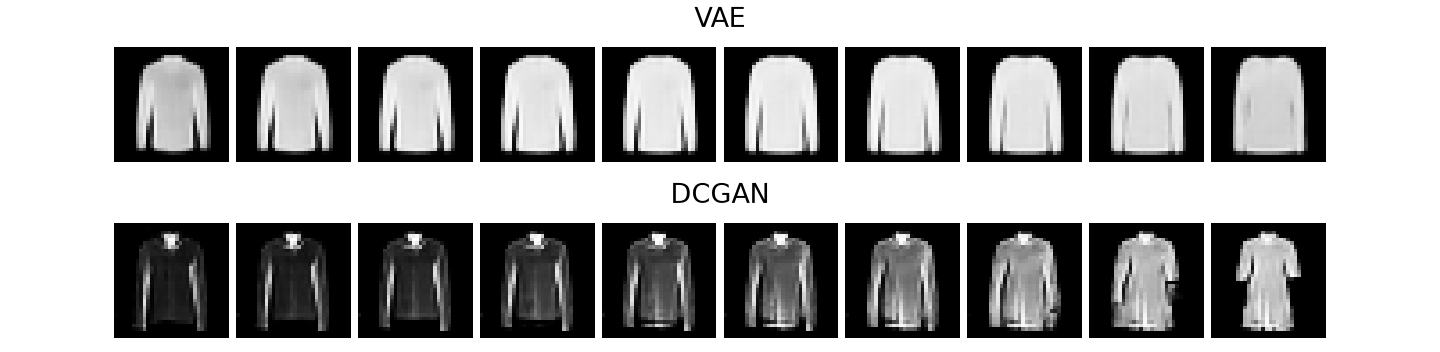
\includegraphics[width=0.97\linewidth]{interpolation.png}
\caption{The first of the 100 interpolation paths for each model.
Images are ordered from the first latent code to the second.}
\label{fig:paths}
\end{figure}
\FloatBarrier

A path can have a low CV even when the overall change is small. For
example, a shirt that gets a little brighter at every step can score
just as well as one that changes shape evenly. This helps explain how
the VAE can have more even steps while the DCGAN covers more of the
variety in the dataset.

We evaluated one saved training run per model. The comparison tells us
how these checkpoints behaved on Fashion-MNIST and leaves open how
much the scores would vary across training runs. The classifier's
features influence the distance and recall scores, and its class
predictions are less reliable on unusual or blurry images. The
DCGAN and VAE also use different Adam settings, so the optimizer
settings may explain part of the difference in addition to the losses.

Class balance tells us how often each clothing label appears. A model
could make the same dress over and over and still produce the expected
share of dresses. Feature recall can pick up missing styles within a
class, such as dresses with different lengths or sleeve shapes, when
those differences show up in the classifier features.

A next step would be to train each model with several seeds and report
the average and spread of the scores. We would use the same classifier,
test images, and evaluation noise for every run. That would show whether
the gap between models is larger than the variation between runs of
the same model.

\section{Conclusion}

Using the same convolutional design, the DCGAN made sharper clothes and
covered more of the real data in this experiment. The VAE made smoother
changes along the latent paths. We expected stronger edges from the
DCGAN, but the gain in recall was more interesting. In this comparison,
the sharper samples also captured more of the variety in the reference
images. Looking at the class chart and the failure examples helped us
understand what the scores were measuring.

\clearpage
\begin{thebibliography}{99}

\bibitem{kingma2014}
D.~P. Kingma and M.~Welling.
\href{https://arxiv.org/abs/1312.6114}{\emph{Auto-Encoding Variational Bayes}}.
ICLR, 2014.

\bibitem{goodfellow2014}
I.~Goodfellow et al.
\href{https://arxiv.org/abs/1406.2661}{\emph{Generative Adversarial Nets}}.
NeurIPS, 2014.

\bibitem{radford2016}
A.~Radford, L.~Metz, and S.~Chintala.
\href{https://arxiv.org/abs/1511.06434}{\emph{Unsupervised Representation
Learning with Deep Convolutional Generative Adversarial Networks}}.
ICLR, 2016.

\bibitem{xiao2017}
H.~Xiao, K.~Rasul, and R.~Vollgraf.
\href{https://arxiv.org/abs/1708.07747}{\emph{Fashion-MNIST: a Novel Image
Dataset for Benchmarking Machine Learning Algorithms}}.
2017.

\bibitem{pytorch}
A.~Paszke et al.
\href{https://arxiv.org/abs/1912.01703}{\emph{PyTorch: An Imperative Style,
High-Performance Deep Learning Library}}.
NeurIPS, 2019.

\bibitem{torchvision}
PyTorch project.
\href{https://github.com/pytorch/vision}{\emph{Torchvision}}.

\bibitem{adam}
D.~P. Kingma and J.~Ba.
\href{https://arxiv.org/abs/1412.6980}{\emph{Adam: A Method for Stochastic
Optimization}}.
ICLR, 2015.

\bibitem{heusel2017}
M.~Heusel et al.
\href{https://arxiv.org/abs/1706.08500}{\emph{GANs Trained by a Two
Time-Scale Update Rule Converge to a Local Nash Equilibrium}}.
NeurIPS, 2017.

\bibitem{kynkaanniemi2019}
T.~Kynk\"a\"anniemi et al.
\href{https://arxiv.org/abs/1904.06991}{\emph{Improved Precision and Recall
Metric for Assessing Generative Models}}.
NeurIPS, 2019.

\bibitem{pechpacheco2000}
J.~L. Pech-Pacheco, G.~Crist\'obal, J.~Chamorro-Mart\'inez, and
J.~Fern\'andez-Valdivia.
\href{https://doi.org/10.1109/ICPR.2000.903548}{\emph{Diatom Autofocusing
in Brightfield Microscopy: A Comparative Study}}.
ICPR, 2000.

\bibitem{white2016}
T.~White.
\href{https://arxiv.org/abs/1609.04468}{\emph{Sampling Generative Networks}}.
2016.

\end{thebibliography}
\end{document}

